\documentclass[10pt,twocolumn,letterpaper]{article}

\usepackage{cvpr}
\usepackage{times}
\usepackage{booktabs}
\usepackage{indentfirst}
\usepackage{epsfig}
\usepackage{float}
\usepackage{amsmath}
\usepackage{picinpar,graphicx}
\usepackage[breaklinks=true,bookmarks=false,colorlinks,
            linkcolor=red,
            anchorcolor=blue,
            citecolor=green,
            backref=page]{hyperref}

\cvprfinalcopy % *** Uncomment this line for the final submission
\def\cvprPaperID{****} % *** Enter the CVPR Paper ID here
\def\httilde{\mbox{\tt\raisebox{-.5ex}{\symbol{126}}}}


\begin{document}

%%%%%%%%% TITLE
\title{Deep Depth Completion of a Single RGB-D Image}

\author{Wenjie Niu\\\\ July 12,2018}

\maketitle
\begin{abstract}
The goal of the paper is to complete the depth channel of an RGB-F image. Commodity-grade depth cameras often fail to sense depth for shiny, bright, transparent, and distant surfaces. To address the problem, the paper train a deep network that takes an RGB image as input and predicts dense surface normals and occlusion bounfaries. \par
\end{abstract}


%%%%%%%% BODY TEXT
\section{Introduction}
Depth sensing has become pervasive in applicationa as diverse as automomous drivig, augemented reality, and scene reconstruction. Despite recent advances in depth sensing technology, commodity-level RGB-D cameras like Microsoft Kinect, Intel RealSense, and Google Tango still produce depth images with missing data when surfaces are too glossy, bright, thin, close, or far from the camera. These problem appear when rooms are large, surfaces are shiny, and strong lighting is abundant-\emph{e.g.}, in museums, hospitals, classrooms, stores, \emph{etc}. Even in homes, depth images often are missing more than 50\% of the pixels(Figure~\ref{fig:Depth})

\begin{figure}[!htp]
\begin{center}
   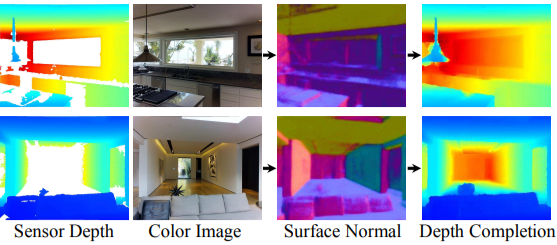
\includegraphics[width=1\linewidth]{DepthCompletion.png}
\end{center}
   \caption{\textbf{Depth Completion.} We fill in large missing areas in the depth channel of an RGB-D image by predicting normals from color and then solving for completed depths~\cite{Zhang_2018_CVPR}.}
\label{fig:Depth}
\end{figure}

\begin{figure*}
\begin{center}
   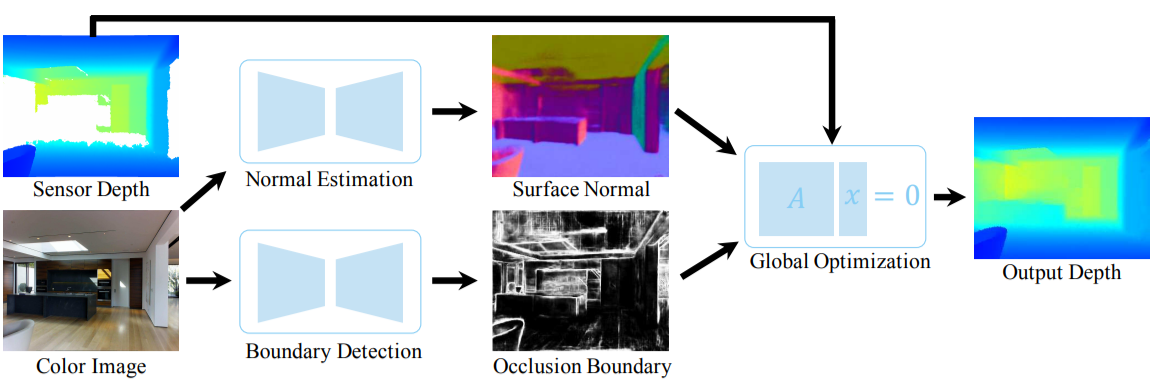
\includegraphics[width=1\linewidth]{Systempipeline.png}
\end{center}
   \caption{\textbf{System pipeline.} Given an input RGB-D image, we predict surface normals and occlusion boundaries from color, and then solve for the output depths with a global linear optimization regularized by the input depth\cite{Zhang_2018_CVPR}.}
\label{fig:System}
\end{figure*}

Though depth inpainting has received a lot of attention over the past two decades\cite{Uhrig2017Sparsity}, it has generally been addressed with hand-tuned methods that fill holes by extrapolating boundary surfaces~\cite{Matsuo2015Depth} or with Markovian images synthesis~\cite{Doria_2012_CVPRW}. Never methods have been proposed to estimate depth de novo from color using deep networks~\cite{Eigen2014Depth}. The solution is to provide the network with only color images as input(Figure~\ref{fig:System}).\par


\section{Related Work}
\textbf{Depth estimation}. Depth estimation from a monocular color image is a long-standing problem in computer vision. Classic methods include shape-from-shading and shape-from-defocus. Other early methods were based on hand-tuned models and/or assumptions about surface orientations. Newer methods treat depth estimation as a machine learning problem, most recently using deep networks.\par
\textbf{Depth inpainting.}Many methods have been proposed for filling holes in depth channels of RGB-D images, including ones that employ smoothness priors, fast marching methods, Navier-Stokes, anisotropic diffusion, background surface extrapolation, color-depth edge alignment, low-rank matrix completion, tensor voting, Mumford-Shah functional optimization, joint optimization with other properties of intrinsic images, and patch-based image synthesis. Recently, methods have been proposed for inpainting color images with auto-encoders and GAN architectures. However, prior work has not investigated how to use those methods for inpainting of depth images. This problem is more difficult due to the absence of strong features in depth images and the lack of large training datasets, an issue addressed in this paper.\par
\textbf{Depth super-resolution.}Several methods have been proposed to improve the spatial resolution of depth images using high-resolution color. They have exploited a variety of approaches, including Markov random fields, shape-from-shading, segmentation, and dictionary methods. Although some of these techniques may be used for depth completion, the challenges of super-resolution are quite different – there the focus is on improving spatial resolution, where low-resolution measurements are assumed to be complete and regularly sampled. In contrast, our focus is on filling holes, which can be quite large and complex and thus require synthesis of large-scale content.\par
\textbf{Depth reconstruction from sparse samples.}Other work has investigated depth reconstruction from color images augmented with sparse sets of depth measurements.\par


%-------------------------------------------------------------------------

{\small
\bibliographystyle{ieee}
\bibliography{DeepDepthCompletionofaSingleRGB-DImage}
}

\end{document}
